\documentclass[10pt]{beamer}

\usepackage[utf8]{inputenc}
\usepackage{pgfpages}
\usepackage{dirtree}
\setbeameroption{show notes on second screen =left} %hide nodes, show only notes, show notes on second screen = left.
\setbeamertemplate{note page}[plain]
\AtEndNote{\vfill \begin{center} mm:hh \end{center}}
\newcommand{\notedir}[1] {
  \note{\dirtree{#1}}}
\def \ion {$^{\circ}$ }
\usepackage{tcolorbox}
\usepackage{tikz}
\usepackage{tikz-3dplot}
\usetikzlibrary{intersections,calc}
\usepackage{amsmath}
\usepackage{graphicx}
\usepackage{cases}
\def \heart {\textcolor{blue}{$\heartsuit$} }
\def \C {$\mathcal{C}$}
\def \orthog {\underline{\perp}}
\def\arcos{\operatorname{arccos}}
\tcbset{%
	basic/.style={colframe=black,
		      colback=white,
		      top= 0mm,
		      bottom = 2mm,
		      boxsep=0mm
		      }
}
\tikzset{
    invisible/.style={opacity=0},
    visible on/.style={alt={#1{}{invisible}}},
    alt/.code args={<#1>#2#3}{%
      \alt<#1>{\pgfkeysalso{#2}}{\pgfkeysalso{#3}} % \pgfkeysalso doesn't change the path
    },
  }

    
\begin{document}  
    \beamertemplatenavigationsymbolsempty
    \setlength{\abovedisplayskip}{0pt}
    \setlength{\belowdisplayskip}{0pt}
    \frame{
	  
	  \frametitle{Q4 Juillet 2001.}
	  On considère un tétraèdre $ABCD$ régulier (c’est-à-dire dont tous les côtés sont
	  égaux). Soit $E$ le milieu du côté $[C, D]$.
	  \renewcommand{\theenumi}{\alph{enumi})}
	  \begin{enumerate}
	   \item Montrer que la droite $CD$ est perpendiculaire au plan $ABE$.
	   \item Montrer que la hauteur du triangle $ABE$ issue de $A$ est perpendiculaire à la
		face $BCD$ et que la hauteur du triangle $ABE$ issue de $B$ est perpendiculaire
		à la face $ACD$.
	   \item Montrer que les pieds des hauteurs du tétraèdre sont les orthocentres des faces
		 correspondantes.
	   \item En déduire que les quatre hauteurs du tétraèdre sont concourantes. 
	  \end{enumerate}

	  
	  \vfill
	  
	  \pause
	  % hypothèses et thèse
	  \begin{tcolorbox}[basic] 
	      \begin{columns}[t]
		 
		 \column{.5\textwidth}\centering
		      
		      \underline{Hypothèses} 
		      \begin{itemize}
		      \item $ABCD$ régulier,
		      \item $|CE|=|ED|$.
		      \end{itemize}

		  
		  \column{.5\textwidth}\centering
		      
		      \underline{Thèses} \\
		      \smallskip
		      \begin{enumerate}
		       
				     \item $CD\bot ABE$,
				     \item $AA'\bot BCD$ et
				       	   $BB'\bot ACD$,
				     \item $A',B',C',D'$ orthocentres,
				     \item $AA',BB',CC', DD'$ concourantes.
		      \end{enumerate}
		      {\small $A',B',C',D'$ pied des hauteurs.} 
		
	      \end{columns}
	  \end{tcolorbox}
    \notedir{%
	.1 Enoncé.
	.2 Hypothèses (non visibles sur le dessin)..
	.2 Thèse : traduction mathématique..
	.3 $A',B',C',D'$ pied des hauteurs..
	.2 Grand dessin.. 
	}
    }

    \frame{ 
	  % résolution ex1
	  \begin{columns}[t]
		\column{.52\textwidth}\centering 
			
			\underline{Dessin}\\
			\vspace{-2mm}	  
				  \begin{figure}[h]
				  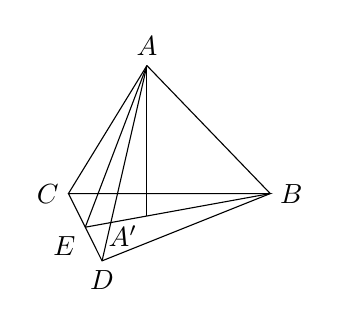
\begin{tikzpicture}[scale=0.78]
				  %AXES
				  %\draw[->] (0,0,-3) -- (0,0,3) coordinate[label=below right:$z$]();
				  %\draw[->] (0,-3,0) -- (0,3,0) coordinate[label=above left:$y$]();
				  %\draw[->] (-3,0,0) -- (3,0,0) coordinate[label=above left:$x$]();
				  %TETRAEDRE et E
				  \coordinate[label=above:$A$] (A) at (0,2.449,0);
				  \coordinate[label=right:$B$] (B) at (1.64317,0,-0.948683);
				  \coordinate[label=left:$C$] (C) at (-1.64317,0,-0.948683);				  
				  \coordinate[label=below:$D$] (D) at (0,0,1.89737);
				  \draw (B) -- (C) -- (D) coordinate[pos=0.5,label=below left:$E$](E) -- cycle;
				  \draw (A) -- (B);
				  \draw (A) -- (C);
				  \draw (A) -- (D);	
				  %AE et EB
				  \draw (A) --(E);
				  \draw (B) -- (E);
				  %A'
				  \coordinate[label=below left:$A'$](A') at (0,0);
				  %AA'
				  \draw (A) -- (A');
				  \end{tikzpicture}
				  \end{figure}
				 \vspace{-3.5mm} 
				  \begin{tcolorbox}[basic]\centering 				      
				    \smallskip
				    \underline{Hypothèses} 
				    \begin{enumerate}
				    \item $ABCD$ régulier,
				    \item $|CE|=|ED|$.
				    \end{enumerate}
							      
				    \underline{Thèses} \\
				    \renewcommand{\theenumi}{\alph{enumi})}
				     \begin{enumerate}
				     \item $CD\bot ABE$,
				     \item $AA'\bot BCD$ et
				       	   $BB'\bot ACD$,
				     \item $A',B',C',D'$ orthocentres,
				     \item $AA',BB',CC', DD'$ concourantes.
				     \end{enumerate}				  
				  \end{tcolorbox}
		
		
		\column{.5\textwidth}\centering
		
		\underline{Résolution}\\ \flushleft
		
		\begin{enumerate}
		\item $ACD,BCD$ $\Delta$ equilatéraux,
		\item $EA$ médiane de $ACD$ \\
		      $EB$ médiane de $BCD$.
		\end{enumerate}	\medskip
		\textcolor{blue}{$\heartsuit_1$} Les droites remarquables d'un $\Delta$ équilatéral sont confondues. \\ \medskip
		$CD\bot EA,CD\bot EB\rightarrow CD\bot ABE$. \\ \hfill$\qed(a)$ \\
		\centering\noindent\rule{2cm}{0.4pt}\flushleft 
		$AA'\bot EB$ car hauteur, \\
		$AA'\orthog CD$ car $AA'\in ABE$, \\
		$AA'\bot BCD$. \\
		\begin{enumerate}
		 \item Propriété montrée pour un sommet est vraie pour tous les autres grâce à la symétrie.
		\end{enumerate}
		$BB'\bot ACD$. \\ \hfill $\qed(b)$ \\
		\centering\noindent\rule{2cm}{0.4pt}		   
	   \end{columns}
	   \notedir{%
	   .1 Prouver thèses.
	   .2 $CD\bot ABE$.
	   .3 Elément de théorie.
	   .4 Droite $\bot$ à plan si $\orthog$ 2 droites sécantes du plan..
	   .3 Résolution..
	   .4 Droites remarquables d'un $\Delta$ confondues..
	   .5 Application à $\Delta ACD,\Delta BCD$.
	   .6 $EA,EB$ médianes $\rightarrow EA,EB$ hauteurs..
	   .6 $CD\bot EA,EB \rightarrow CD\bot ABE$..
	   .2 $AA'\bot BCD$ et $BB'\bot ACD$.
	   .3 Elément de théorie.
	   .4 Droite $\bot$ à plan si $\orthog$ 2 droites sécantes du plan..
	   .3 Résolution..
	   .4 $AA'\bot EB$ car hauteur..
	   .4 Droite $\bot$ à plan $\rightarrow$ droite $\orthog$ à tt.~droites du plan..
	   .5 Application à $CD$ et $ABE$ $\rightarrow AA' \orthog CD$..
	   .4 $\rightarrow AA'\bot EB, AA'\orthog CD \rightarrow AA'\bot BCD$..
	   .4 Par symétrie tétraèdre régulier, $BB'\bot ACD$..
	   }
          }  	
          
    \frame{ 
	  % résolution ex1
	  \begin{columns}[t]
		\column{.53\textwidth}\centering 
			
			\underline{Dessin}\\
			\vspace{-2mm}	  
				  \begin{figure}[h]
				  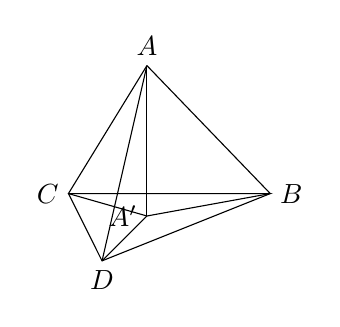
\begin{tikzpicture}[scale=0.78]
				  %AXES
				  %\draw[->] (0,0,-3) -- (0,0,3) coordinate[label=below right:$z$]();
				  %\draw[->] (0,-3,0) -- (0,3,0) coordinate[label=above left:$y$]();
				  %\draw[->] (-3,0,0) -- (3,0,0) coordinate[label=above left:$x$]();
				  %TETRAEDRE et E
				  \coordinate[label=above:$A$] (A) at (0,2.449,0);
				  \coordinate[label=right:$B$] (B) at (1.64317,0,-0.948683);
				  \coordinate[label=left:$C$] (C) at (-1.64317,0,-0.948683);				  
				  \coordinate[label=below:$D$] (D) at (0,0,1.89737);
				  \draw (B) -- (C) -- (D) -- cycle;
				  \draw (A) -- (B);
				  \draw (A) -- (C);
				  \draw (A) -- (D);	
				  				  
				  %A'
				  \coordinate[label=left:$A'$](A') at (0,0);
				  %AA'
				  \draw (A) -- (A');
				  %A'C,A'D, A'B%
				  \draw (A')--(B);
				  \draw (A') -- (C);
				  \draw (A') -- (D);
				  \end{tikzpicture}
				  \end{figure}
				 \vspace{-3.5mm} 
				  \begin{tcolorbox}[basic]\centering 				      
				    \smallskip
				    \underline{Hypothèses} 
				    \begin{enumerate}
				    \item $ABCD$ régulier,
				    \item $|CE|=|ED|$.
				    \end{enumerate}
							      
				    \underline{Thèses} \\
				    \renewcommand{\theenumi}{\alph{enumi})}
				     \begin{enumerate}
				     \item $CD\bot ABE$,
				     \item $AA'\bot BCD$ et
				       	   $BB'\bot ACD$,
				     \item $A',B',C',D'$ orthocentres,
				     \item $AA',BB',CC', DD'$ concourantes.
				     \end{enumerate}				  
				  \end{tcolorbox}
		
		
		\column{.52\textwidth}\flushleft
		
		\begin{align*} 
			  &|AB|= |AC|=|AD|, \\[0.5em]
			  &AA'\bot BCD :  \\[-0.3em]
			  &\widehat{BAA'}=\widehat{CAA'}=\widehat{DAA'} =\arcos\dfrac{|AA'|}{|AB|}, \\		
		\end{align*}
		\vspace{-8mm}
		
		\textcolor{blue}{$\heartsuit_2$} Des $\Delta$ sont isométriques s'ils ont un angle de même mesure entre 2 côtés de mêmes longueurs. \\ \medskip
		$\Delta BAA',\Delta CAA',\Delta DAA'$ isométriques. \\
		\begin{align*}
		A'=& \text{ centre cercle circonscrit,} \\
		  =& \text{ orthocentre. (\textcolor{blue}{$\heartsuit_1$})} 
		\end{align*}
		\begin{enumerate}
		 \item Propriété montrée pour un sommet est vraie pour tous les autres grâce à la symétrie.\\ \hfill $\qed(c)$
		\end{enumerate}
		\centering\noindent\rule{2cm}{0.4pt}	
			   
	   \end{columns}
	   \notedir{%
	   .1 Prouver thèses.
	   .2 $A',B',C',D'$ orthocentres.~(commencer par $A'$).
	   .3 Elément de théorie.
	   .4 Les droites remarquables d'un $\Delta$ équilatéral sont\\ \hspace{5mm} confondues..
	   .5 Montrer que $A'$ est centre cercle circonscrit à $\Delta BCD$..
	   .3 Résolution..
	   .4 $\Delta BAA',\Delta CAA',\Delta DAA'$ isométriques car.
	   .5 2 cotés ($AA'$ et arête) et un angle en commun..
	   .6 $|A'B| = |A'C| = |A'D|\rightarrow A'$ centre cercle..
	   .7 $A'$ orthocentre..
	   .4 Par symétrie du tétraèdre régulier, vrai pour $B',C',D'$..
	   }
          }  
    
   \frame{ 
	  % résolution ex1
	  \begin{columns}[t]
		\column{.52\textwidth}\centering 
			
			\underline{Dessin}\\
			\vspace{-2mm}	  
				  \begin{figure}[h]
				  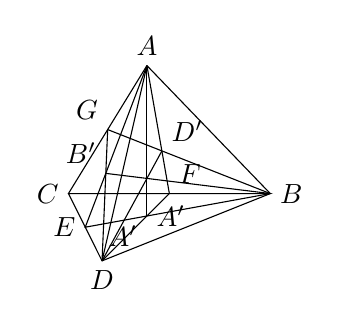
\begin{tikzpicture}[scale=0.78]
				  %AXES
				  %\draw[->] (0,0,-3) -- (0,0,3) coordinate[label=below right:$z$]();
				  %\draw[->] (0,-3,0) -- (0,3,0) coordinate[label=above left:$y$]();
				  %\draw[->] (-3,0,0) -- (3,0,0) coordinate[label=above left:$x$]();
				  %TETRAEDRE et E
				  \coordinate[label=above:$A$] (A) at (0,2.449,0);
				  \coordinate[label=right:$B$] (B) at (1.64317,0,-0.948683);
				  \coordinate[label=left:$C$] (C) at (-1.64317,0,-0.948683);				  
				  \coordinate[label=below:$D$] (D) at (0,0,1.89737);
				  \draw (B) -- (C) -- (D) -- cycle;
				  \draw (A) -- (B);
				  \draw (A) -- (C);
				  \draw (A) -- (D);	
				  				  
				  %A',B',C',D'
				  \coordinate[](A') at (0,0);
				  \coordinate[](B') at ($0.333*(A)+0.333*(C)+0.333*(D)$);
				  %\coordinate[label=above right:$C'$](C') at ($0.333*(A)+0.333*(B)+0.333*(D)$);
				  \coordinate[](D') at ($0.333*(A)+0.333*(B)+0.333*(C)$);
				  
				  %E,F,G
				  \coordinate[] (E) at ($0.5*(C)+0.5*(D)$); 
				  \coordinate[] (F) at ($0.5*(C)+0.5*(B)$);
				  \coordinate[] (G) at ($0.5*(A)+0.5*(C)$);
				  %AA',BB',CC',DD'
				  \draw[visible on=<1>] (A) -- (A') node[below left] {$A'$};
				  \draw[visible on=<{2,4}>] (A) -- (A') node[right] {$A'$};
				  \draw[visible on=<{1,3,4}>] (B) -- (B') node[above left]{$B'$};
				  \draw[visible on=<2-4>] (D) -- (D') node[above right]{$D'$}; 
				  \draw[visible on=<1>] (A) -- (E) node[left]{$E$} -- (B);
				  \draw[visible on=<2>] (A) -- (F) node[above right]{$F$}-- (D);
				  \draw[visible on=<3>] (B) -- (G) node[above left]{$G$}-- (D);
				  \end{tikzpicture}
				  \end{figure}
				 \vspace{-3.5mm} 
				  \begin{tcolorbox}[basic]\centering 				      
				    \smallskip
				    \underline{Hypothèses} 
				    \begin{enumerate}
				    \item $ABCD$ régulier,
				    \item $|CE|=|ED|$.
				    \end{enumerate}
							      
				    \underline{Thèses} \\
				    \renewcommand{\theenumi}{\alph{enumi})}
				     \begin{enumerate}
				     \item $CD\bot ABE$,
				     \item $AA'\bot BCD$ et
				       	   $BB'\bot ACD$,
				     \item $A',B',C',D'$ orthocentres,
				     \item $AA',BB',CC', DD'$ concourantes.
				     \end{enumerate}				  
				  \end{tcolorbox}
		
		
		\column{.5\textwidth}\flushleft
		\onslide<+-> $AA'\nmid BB'$ (hauteurs $\Delta ABE$) \\
		\onslide<+-> $AA'\nmid DD'$ (hauteurs $\Delta ADF$) \\
		\onslide<+-> $BB'\nmid DD'$ (hauteurs $\Delta BDG$) \\
		\onslide<+->\begin{numcases}{}X= AA' \cap BB', \label{eq:1}\\
					      Y= AA' \cap DD', \label{eq:2}\\
					      Z= BB' \cap DD'. \label{eq:3} 
			    \end{numcases} \smallskip
		
		 
		\begin{align*}
		Y \in& AA' \subset AA'B, \\
		Z \in& BB' \subset AA'B, \\
		\text{et }&  Y,Z \in DD', \\[1em]				
			    Y =& Z  =DD' \cap AA'B. \\[1.5em]		
			    Y =& AA' \cap DD' = BB' \cap DD', (\ref{eq:2}=\ref{eq:3}) \\
			      =& AA' \cap BB', \text{(transitivité)}\\
			      =& X.\\
			    X =& Y = Z. 	      
		\end{align*}
		
			   
	   \end{columns}
	   \notedir{%
	   .1 Prouver thèses.
	   .2 $AA',BB',CC', DD'$ concourantes.~(commencer par $AA',BB',CC'$).
	   .3 Elément de théorie.
	   .4 3 droites non coplanaires sécantes 2 à 2 sont concourantes (à prouver car non vu)..
	   .3 Résolution.
	   .4 Les droites sont sécantes 2 à 2 car hauteurs $\Delta$..
	   .4 Former un plan avec 2 droites, $AA'$ et $BB'$.
	   .5 L'intersect\ion de $DD'$ avec $AA'$ et celle avec $BB'$\\ \hspace{5mm} appartiennent au plan et à $DD'$.
	   .6 Ces deux intersect\ion sont confondues car\\ \hspace{5mm} point de percée de $DD'$ ds.~plan est \\ \hspace{5mm} unique..
	   .7 Ce point de percée appartient à la fois à $AA',BB',DD' \rightarrow$ droites concourantes..
	   }
          }
          
       \frame{ 
	  % résolution ex1
	  \begin{columns}[t]
		\column{.52\textwidth}\centering 
			
			\underline{Dessin}\\
			\vspace{-2mm}	  
				  \begin{figure}[h]
				  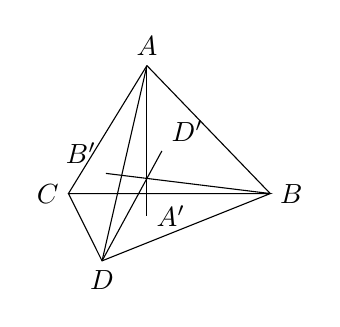
\begin{tikzpicture}[scale=0.78]
				  %AXES
				  %\draw[->] (0,0,-3) -- (0,0,3) coordinate[label=below right:$z$]();
				  %\draw[->] (0,-3,0) -- (0,3,0) coordinate[label=above left:$y$]();
				  %\draw[->] (-3,0,0) -- (3,0,0) coordinate[label=above left:$x$]();
				  %TETRAEDRE et E
				  \coordinate[label=above:$A$] (A) at (0,2.449,0);
				  \coordinate[label=right:$B$] (B) at (1.64317,0,-0.948683);
				  \coordinate[label=left:$C$] (C) at (-1.64317,0,-0.948683);				  
				  \coordinate[label=below:$D$] (D) at (0,0,1.89737);
				  \draw (B) -- (C) -- (D) -- cycle;
				  \draw (A) -- (B);
				  \draw (A) -- (C);
				  \draw (A) -- (D);	
				  				  
				  %A',B',C',D'
				  \coordinate[](A') at (0,0);
				  \coordinate[](B') at ($0.333*(A)+0.333*(C)+0.333*(D)$);
				  %\coordinate[label=above right:$C'$](C') at ($0.333*(A)+0.333*(B)+0.333*(D)$);
				  \coordinate[](D') at ($0.333*(A)+0.333*(B)+0.333*(C)$);
				  
				
				  %AA',BB',CC',DD'
				  \draw (A) -- (A') node[right] {$A'$};
				  \draw (B) -- (B') node[above left]{$B'$};
				  \draw (D) -- (D') node[above right]{$D'$}; 
				
				  \end{tikzpicture}
				  \end{figure}
				 \vspace{-3.5mm} 
				  \begin{tcolorbox}[basic]\centering 				      
				    \smallskip
				    \underline{Hypothèses} 
				    \begin{enumerate}
				    \item $ABCD$ régulier,
				    \item $|CE|=|ED|$.
				    \end{enumerate}
							      
				    \underline{Thèses} \\
				    \renewcommand{\theenumi}{\alph{enumi})}
				     \begin{enumerate}
				     \item $CD\bot ABE$,
				     \item $AA'\bot BCD$ et
				       	   $BB'\bot ACD$,
				     \item $A',B',C',D'$ orthocentres,
				     \item $AA',BB',CC', DD'$ concourantes.
				     \end{enumerate}				  
				  \end{tcolorbox}
		
		
		\column{.5\textwidth}\flushleft
		$AA',BB',DD'$ sont concourantes. \\ \medskip
		De la même façon : \\ \medskip
		$AA',BB',CC'$ sont concourantes. \\ \bigskip
		Ainsi $AA',BB',CC',DD'$ sont concourantes. \hfill $\qed(d)$
			   
	   \end{columns}
	   \notedir{%
	   .1 Suite de $AA',BB',CC', DD'$ concourantes.
	   .2 De la même façon, $AA',BB',CC'$ sont concourantes..
	   .3 L'intersect\ion de $AA',BB'$ appartient à $DD'$ et à $CC'$.
	   .4 $\rightarrow AA',BB',CC',DD'$ concourantes..
	   }
          }
  
  
\end{document}
